\section{Gradient Descent}
\frame{\tableofcontents[currentsection, hideothersubsections]}

\begin{frame}
\frametitle{Gradient Descent}

Recall:\\
\begin{itemize}
\item hypotheses as vectors $\mathbf{w}$ that come from a convex hypothesis class, $\mathcal{H}$
\item the goal of learning is to minimize the risk function $L_D(\mathbf{w})$;\\
      \textbf{not} the empirical risk $L_S (h)$
\end{itemize}

\begin{figure}
    \centering
    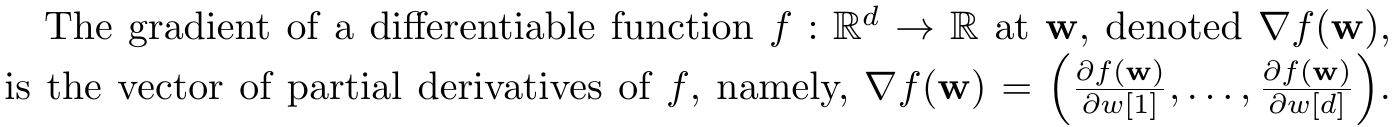
\includegraphics[scale=0.30]{grad_def_p185}
\end{figure}


\end{frame}

\begin{frame}
\frametitle{Gradient Descent}
Gradient descent:
\begin{itemize}
\item an iterative optimization procedure
\item at each step: \\
    improve the solution by
    taking a step along the negative of the gradient of the function to be minimized at the current point

    \begin{figure}
    \centering
    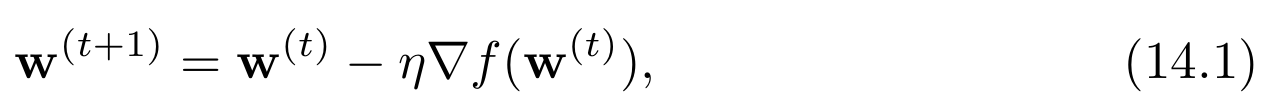
\includegraphics[scale=0.30]{eq_14_1}
    \end{figure}
\item after $T$ iterations, output either
    \begin{itemize}
        \item averaged vector, \textbf{or}
        \item last vector, \textbf{or}
        \item the best performing vector
    \end{itemize}
\end{itemize}

\end{frame}

\begin{frame}
\frametitle{Gradient Descent}
Gradient descent:
\begin{itemize}
\item an iterative optimization procedure
\item at each step: \\
    improve the solution by
    taking a step along the negative of the gradient of the function to be minimized at the current point

    \begin{figure}
    \centering
    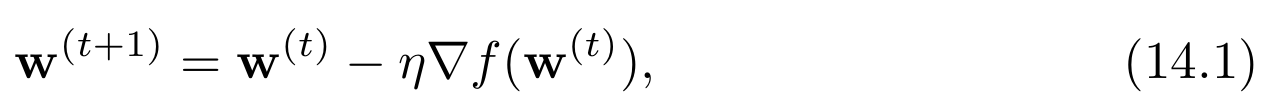
\includegraphics[scale=0.30]{eq_14_1}
    \end{figure}
\item after $T$ iterations, output either
    \begin{itemize}
        \item averaged vector, \textbf{or}
        \item last vector, \textbf{or}
        \item the best performing vector
    \end{itemize}
\end{itemize}

\end{frame}

\begin{frame}
\frametitle{Gradient Descent: Analysis of GD for Convex-Lipschitz Fn}

LET:
\begin{itemize}
\item $\mathbf{w^*}$ be any vector and
\item $B$ be an upper bound on $\parallel \mathbf{w^*} \parallel$
\end{itemize}
\vspace{3mm}

GOAL:\\
to obtain an upper bound on  $f(\bar{\mathbf{w}}) - f(\mathbf{w^*})$,
where $\bar{\mathbf{w}} = \frac{1}{T} \sum_{1}^{T} \mathbf{w}^{(t)}$
\vspace{3mm}

RESULT:\\
From the definition of $\bar{\mathbf{w}}$, and using Jensen's inequality, we obtain:
\begin{figure}
    \centering
    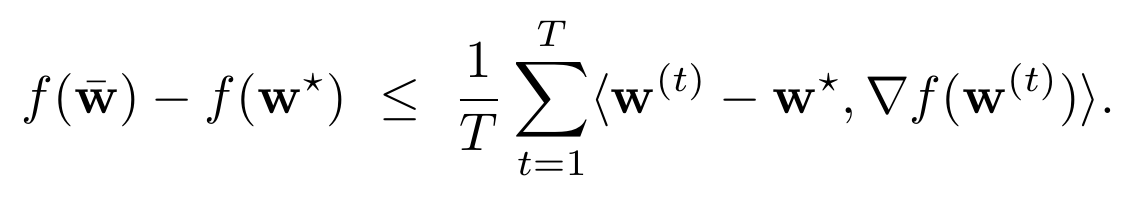
\includegraphics[scale=0.25]{eq_14_3b}
\end{figure}

\end{frame}

\begin{frame}
\frametitle{Gradient Descent: Analysis of GD for Convex-Lipschitz Fn}

\begin{figure}
    \centering
    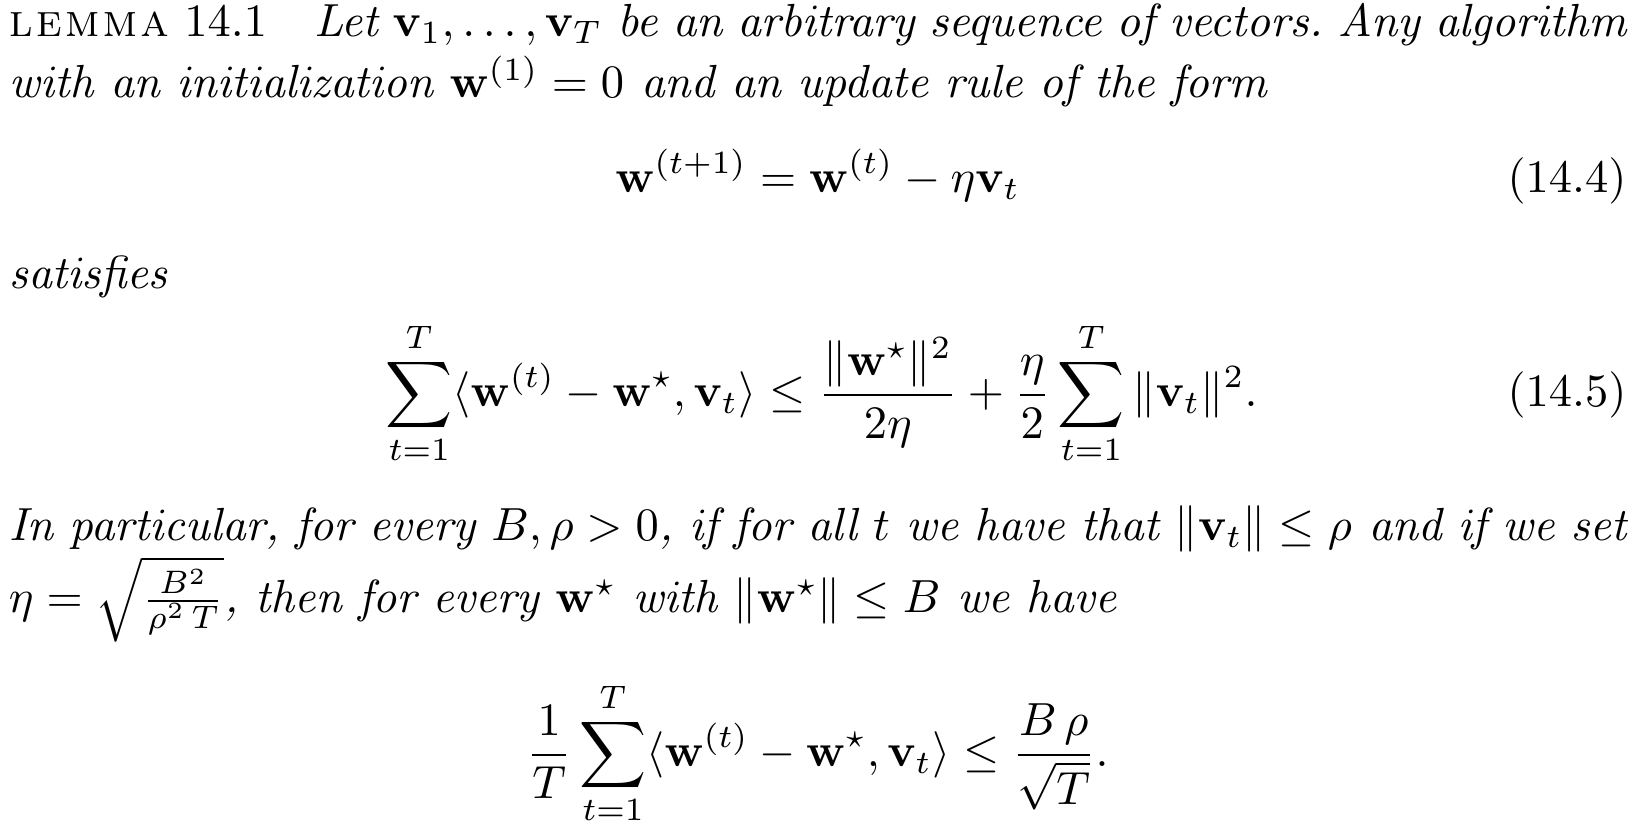
\includegraphics[scale=0.30]{lemma_14_1}
\end{figure}

\end{frame}

\begin{frame}
\frametitle{Gradient Descent: Analysis of GD for Convex-Lipschitz Fn}

\begin{figure}
    \centering
    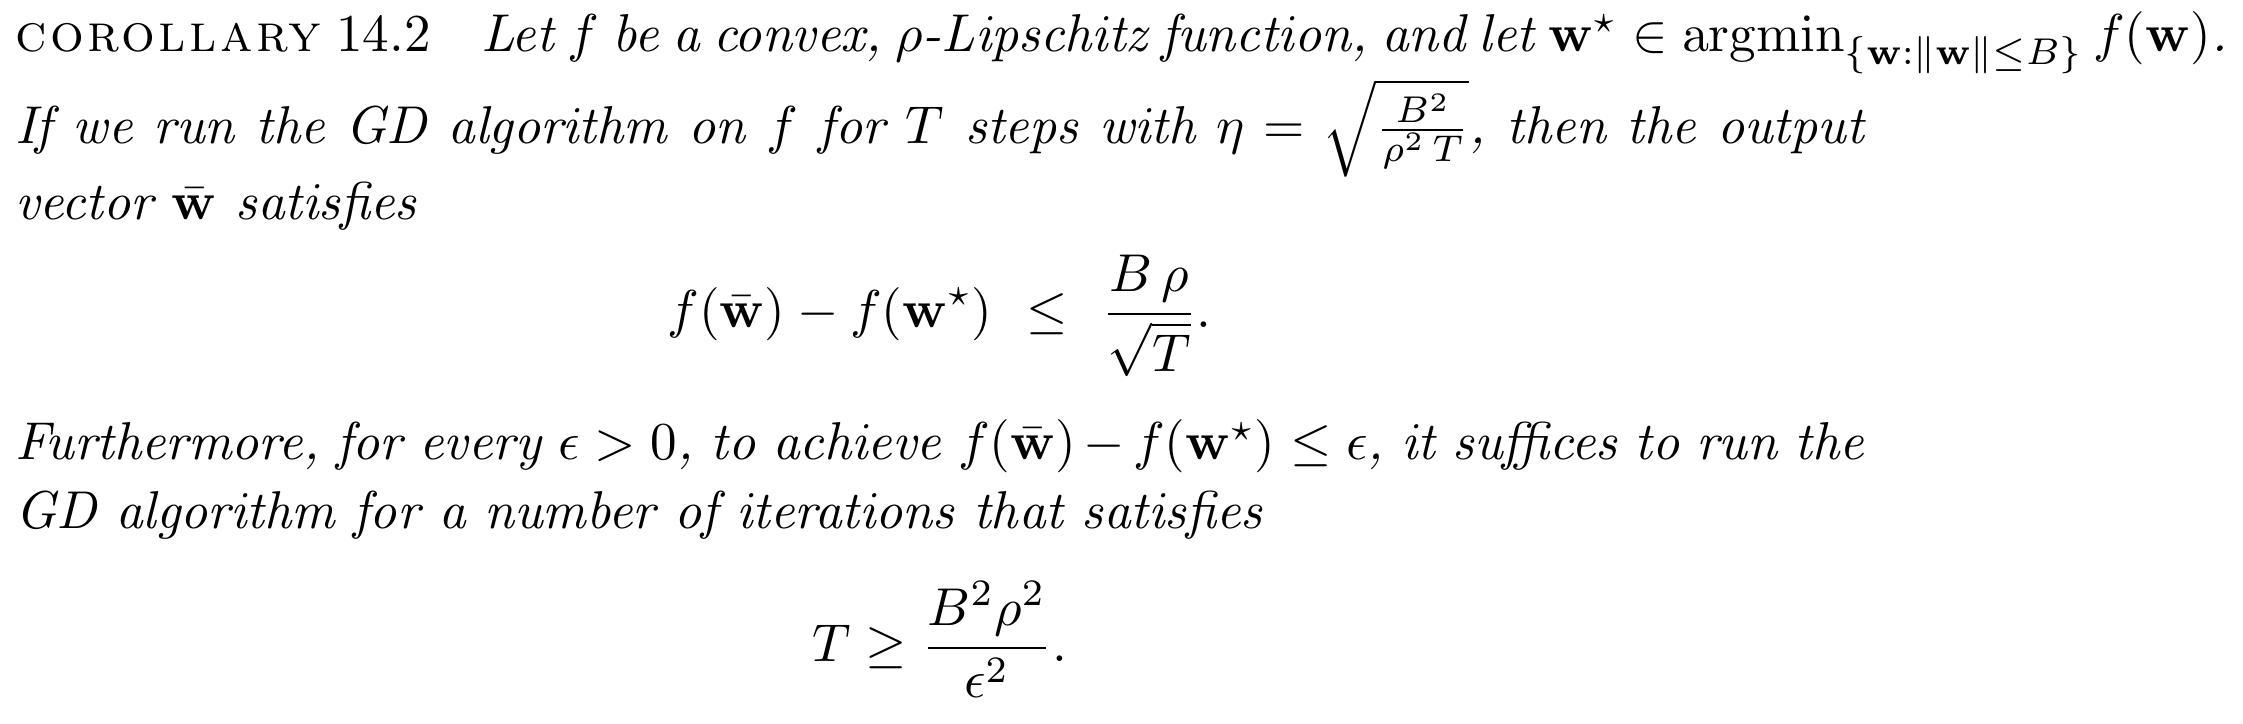
\includegraphics[scale=0.2]{corollary_14_2}
\end{figure}

\end{frame}
